\documentclass[journal=jpcbfk]{achemso}

\usepackage[version=3]{mhchem}
\usepackage[T1]{fontenc}
\newcommand*\mycommand[1]{\texttt{\emph{#1}}}
\newcommand{\todo}[1]{\textcolor{red}{#1}}

\usepackage{rotating}
\usepackage{upgreek}				
\usepackage{xcolor}
\usepackage{booktabs}
\usepackage{multirow}
\usepackage{lmodern}
\usepackage{microtype}
\usepackage{soul}
\usepackage{xr}

\makeatletter
\newcommand*{\addFileDependency}[1]{% argument=file name and extension
  \typeout{(#1)}
  \@addtofilelist{#1}
  \IfFileExists{#1}{}{\typeout{No file #1.}}
}
\makeatother

\newcommand*{\myexternaldocument}[1]{%
    \externaldocument{#1}%
    \addFileDependency{#1.tex}%
    \addFileDependency{#1.aux}%
    \addFileDependency{MANUSCRIPT/#1.tex}%
    \addFileDependency{MANUSCRIPT/#1.aux}%
}

\externaldocument{manuscript}

\author{Peter Heftberger}
\affiliation{Institute of Molecular Biosciences, Biophysics Division, NAWI Graz, University of Graz, Graz 8010, Austria}
%
\author{Matti Javanainen}
\affiliation{Institute of Organic Chemistry and Biochemistry,
Academy of Sciences of the Czech Republic, 
Prague 6, Czech Republic}
\alsoaffiliation{Institute of Biotechnology, University of Helsinki}
\email{matti.javanainen@helsinki.fi}
%
\author{Jesper J. Madsen}
\affiliation{Department of Global Health, College of Public Health}
\alsoaffiliation{University of South Florida}
%
\author{Josef Melcr}
\affiliation{Institute of Organic Chemistry and Biochemistry,
Academy of Sciences of the Czech Republic, 
Prague 6, Czech Republic}
%
\author{Markus Miettinen}
\affiliation{Department of Chemistry, University of Bergen, Norway}
\alsoaffiliation{Computational Biology Unit, Department of Informatics, University of Bergen, Norway}

%
\author{O. H. Samuli Ollila}
\affiliation{Institute of Organic Chemistry and Biochemistry,
Academy of Sciences of the Czech Republic, 
Prague 6, Czech Republic}
\alsoaffiliation{Institute of Biotechnology, University of Helsinki}
\email{samuli.ollila@helsinki.fi}
%
\author{Georg Pabst}
\affiliation{Institute of Molecular Biosciences, Biophysics Division, NAWI Graz, University of Graz, Graz 8010, Austria}
\alsoaffiliation{BioTechMed-Graz, Graz 8010, Austria}
%

\SectionNumbersOn

\renewcommand{\thetable}{S\arabic{table}}%
\renewcommand{\thefigure}{S\arabic{figure}}%
\renewcommand{\thesection}{S\arabic{section}}%
\renewcommand{\thepage}{S\arabic{page}}%


\title{SUPPLEMENTARY INFORMATION FOR\\ 
    NMRlipids III: Lipid--Cholesterol Interactions in Atomistic Resolution Molecular Dynamics Simulations}

\begin{document}

\tableofcontents

\section{Simulation Details}

The force field specific simulation parameters used for each force field are listed in Table~\ref{SItab:params}. The parameter input files (\texttt{.mdp}) are provided in the Zenodo portal (links in the main text). For all simulations, we used an integration time step of 2~fs and the leap-frog integrator of GROMACS. The isothermal--isobaric (NPT) ensemble was used with a temperature of 298~K and a pressure of 1~bar. All simulations were 1~\textmu{}s long, and trajectories were written every 1~ns. The P-LINCS constraint algorithm \cite{hess97,hess07} was used for the bonds noted in Table~\ref{SItab:params}. NMRlipids databank~\cite{NMRlipidsDatabank} ID numbers of simulations are given in table~\ref{IDtable}.

\begin{sidewaystable}[]
\begin{center}
    \caption{\label{SItab:params}%
    Simulation parameters used for different force fields.
    }
    \begin{tabular}{lcccc}
    \toprule
    \textbf{Parameter} & \textbf{CHARMM36} & \textbf{Slipids} & \textbf{Lipid17} & \textbf{MacRog} \\
    \midrule % NB interactions
    Neighbour list type & Verlet \cite{pall2013flexible} & Verlet \cite{pall2013flexible} & Verlet \cite{pall2013flexible} & Verlet \cite{pall2013flexible} \\
    Long-range electrostatics & PME \cite{essman95,darden93} & PME \cite{essman95,darden93} & PME \cite{essman95,darden93} & PME \cite{essman95,darden93} \\
    LJ cut-off & 1.2~nm & 1.4~nm & 0.9~nm & 1.0~nm \\
    LJ modifier & Force switch 1.0--1.2~nm & -- & -- & -- \\
    Dispersion correction & -- & Energy \& pressure \cite{shirts2007accurate} & Energy \& pressure \cite{shirts2007accurate} & Energy \& pressure \cite{shirts2007accurate} \\
    \midrule % P/T control
    Thermostat & Nos\'{e}--Hoover \cite{hoover85,nose84} & Stochastic rescaling \cite{bussi07} & Nos\'{e}--Hoover \cite{hoover85,nose84} & Stochastic rescaling \cite{bussi07} \\
    Time constant ($T$) & 1~ps & 0.5~ps & 1~ps & 0.1~ps \\
    Coupling groups & Lipids \& water & Lipids \& water & Lipids \& water & Lipids \& water \\
    Barostat & Parrinello--Rahman \cite{parrinello1981polymorphic} & Berendsen \cite{berendsen1984molecular} & Parrinello--Rahman \cite{parrinello1981polymorphic} & Parrinello--Rahman \cite{parrinello1981polymorphic} \\
    Coupling type ($P$) & semi-isotropic & semi-isotropic & semi-isotropic & semi-isotropic \\
    Time constant ($P$) & 5~ps & 10~ps & 5~ps & 4~ps\\
    Compressibility & 4.5$\cdot$10$^{-5}$~1/bar & 4.5$\cdot$10$^{-5}$~1/bar & 4.5$\cdot$10$^{-5}$~1/bar & 4.5$\cdot$10$^{-5}$~1/bar \\
    \midrule % Constraints
    Constraints & Bonds with H & All bonds & Bonds with H & All bonds \\
    \midrule 
    Water model & TIPS3P \cite{durell1994solvent}  & TIP3P \cite{jorgensen83} & TIP3P \cite{jorgensen83} & TIP3P \cite{jorgensen83} \\
    FF Source & CHARMM-GUI & CHARMM-GUI & CHARMM-GUI & Refs.~\citenum{Kulig16} \& \citenum{macrogpopc} \\
    Parameter source & CHARMM-GUI & Slipids website & CHARMM-GUI & Refs.~\citenum{Kulig16} \& \citenum{macrogpopc} \\
    \bottomrule
    \end{tabular}
\end{center}
\end{sidewaystable}

\clearpage

\begin{table}[]
\begin{tabular}{ccc}
\textbf{CHARMM36} \\
\toprule
\textbf{System} & \textbf{ID} \\
\midrule
1024POPC\_128CHOL\_57600SOL\_298K  &  426 \\ 
64POPC\_3200SOL\_298K  &  546 \\ 
1024POPC\_896CHOL\_96000SOL\_298K  &  543 \\ 
64POPC\_40CHOL\_5200SOL\_298K  &  620 \\ 
64POPC\_56CHOL\_6000SOL\_298K  &  91 \\ 
1024POPC\_416CHOL\_72000SOL\_298K  &  412 \\ 
1024POPC\_256CHOL\_64000SOL\_298K  &  88 \\ 
256POPC\_64CHOL\_16000SOL\_298K  &  72 \\ 
64POPC\_8CHOL\_3600SOL\_298K  &  109 \\ 
256POPC\_104CHOL\_18000SOL\_298K  &  298 \\ 
64POPC\_16CHOL\_4000SOL\_298K  &  525 \\ 
64POPC\_26CHOL\_4500SOL\_298K  &  393 \\ 
1024POPC\_640CHOL\_83200SOL\_298K  &  550 \\ 
256POPC\_160CHOL\_20800SOL\_298K  &  275 \\ 
256POPC\_224CHOL\_24000SOL\_298K  &  166 \\ 
256POPC\_32CHOL\_14400SOL\_298K  &  119 \\ 
\end{tabular}
\quad
\begin{tabular}{cc}
\textbf{Slipids} \\
\toprule
\textbf{System} & \textbf{ID} \\
\midrule
Slipids\_POPC\_CHOL20\_L  &  691 \\ 
Slipids\_POPC\_CHOL47\_M  &  712 \\ 
Slipids\_POPC\_CHOL29\_S  &  693 \\ 
Slipids\_POPC\_CHOL20\_S  &  692 \\ 
Slipids\_POPC\_CHOL20\_M  &  687 \\ 
Slipids\_POPC\_CHOL11\_S  &  672 \\ 
Slipids\_POPC\_CHOL11\_M  &  681 \\ 
Slipids\_POPC\_L  &  696 \\ 
Slipids\_POPC\_CHOL38\_S  &  661 \\ 
Slipids\_POPC\_M  &  708 \\ 
Slipids\_POPC\_CHOL38\_L  &  670 \\ 
Slipids\_POPC\_S  &  664 \\ 
Slipids\_POPC\_CHOL29\_L  &  709 \\ 
Slipids\_POPC\_CHOL29\_M  &  659 \\ 
Slipids\_POPC\_CHOL11\_L  &  697 \\ 
Slipids\_POPC\_CHOL38\_M  &  668 \\ 
Slipids\_POPC\_CHOL47\_S  &  703 \\ 
Slipids\_POPC\_CHOL47\_L  &  682 \\
\end{tabular}
\quad
\begin{tabular}{cc}
\textbf{Lipid17} \\
\toprule
\textbf{System} & \textbf{ID} \\
\midrule
Lipid17\_POPC\_CHOL29\_M  &  700 \\ 
Lipid17\_POPC\_CHOL47\_L  &  717 \\ 
Lipid17\_POPC\_CHOL11\_L  &  663 \\ 
Lipid17\_POPC\_CHOL29\_L  &  683 \\ 
Lipid17\_POPC\_CHOL20\_S  &  662 \\ 
Lipid17\_POPC\_CHOL47\_M  &  714 \\ 
Lipid17\_POPC\_CHOL38\_S  &  688 \\ 
Lipid17\_POPC\_L  &  684 \\ 
Lipid17\_POPC\_S  &  715 \\ 
Lipid17\_POPC\_CHOL20\_M  &  666 \\ 
Lipid17\_POPC\_M  &  657 \\ 
Lipid17\_POPC\_CHOL29\_S  &  686 \\ 
Lipid17\_POPC\_CHOL38\_L  &  673 \\ 
Lipid17\_POPC\_CHOL47\_S  &  707 \\ 
Lipid17\_POPC\_CHOL11\_S  &  680 \\ 
Lipid17\_POPC\_CHOL20\_L  &  667 \\ 
Lipid17\_POPC\_CHOL38\_M  &  694 \\ 
Lipid17\_POPC\_CHOL11\_M  &  689 \\
\end{tabular}
\quad
\begin{tabular}{cc}
\textbf{MacRog} \\
\toprule
\textbf{System} & \textbf{ID} \\
\midrule
MacRog\_POPC\_CHOL38\_S  &  716 \\ 
MacRog\_POPC\_CHOL29\_L  &  705 \\ 
MacRog\_POPC\_CHOL47\_M  &  699 \\ 
MacRog\_POPC\_CHOL47\_L  &  671 \\ 
MacRog\_POPC\_CHOL20\_L  &  677 \\ 
MacRog\_POPC\_S  &  674 \\ 
MacRog\_POPC\_CHOL20\_M  &  706 \\ 
MacRog\_POPC\_CHOL38\_L  &  698 \\ 
MacRog\_POPC\_CHOL38\_M  &  679 \\ 
MacRog\_POPC\_M  &  675 \\ 
MacRog\_POPC\_L  &  658 \\ 
MacRog\_POPC\_CHOL29\_M  &  655 \\ 
MacRog\_POPC\_CHOL11\_L  &  660 \\ 
MacRog\_POPC\_CHOL11\_S  &  665 \\ 
MacRog\_POPC\_CHOL29\_S  &  690 \\ 
MacRog\_POPC\_CHOL11\_M  &  695 \\ 
MacRog\_POPC\_CHOL47\_S  &  704 \\ 
MacRog\_POPC\_CHOL20\_S  &  702 \\
\end{tabular}
\caption{NMRlipids databank IDs of performed simulations.}\label{IDtable}
\end{table}

\clearpage

\section{Additional Results}

\subsection{Scattering Intensities}

\begin{figure}[htb!]
    \centering
    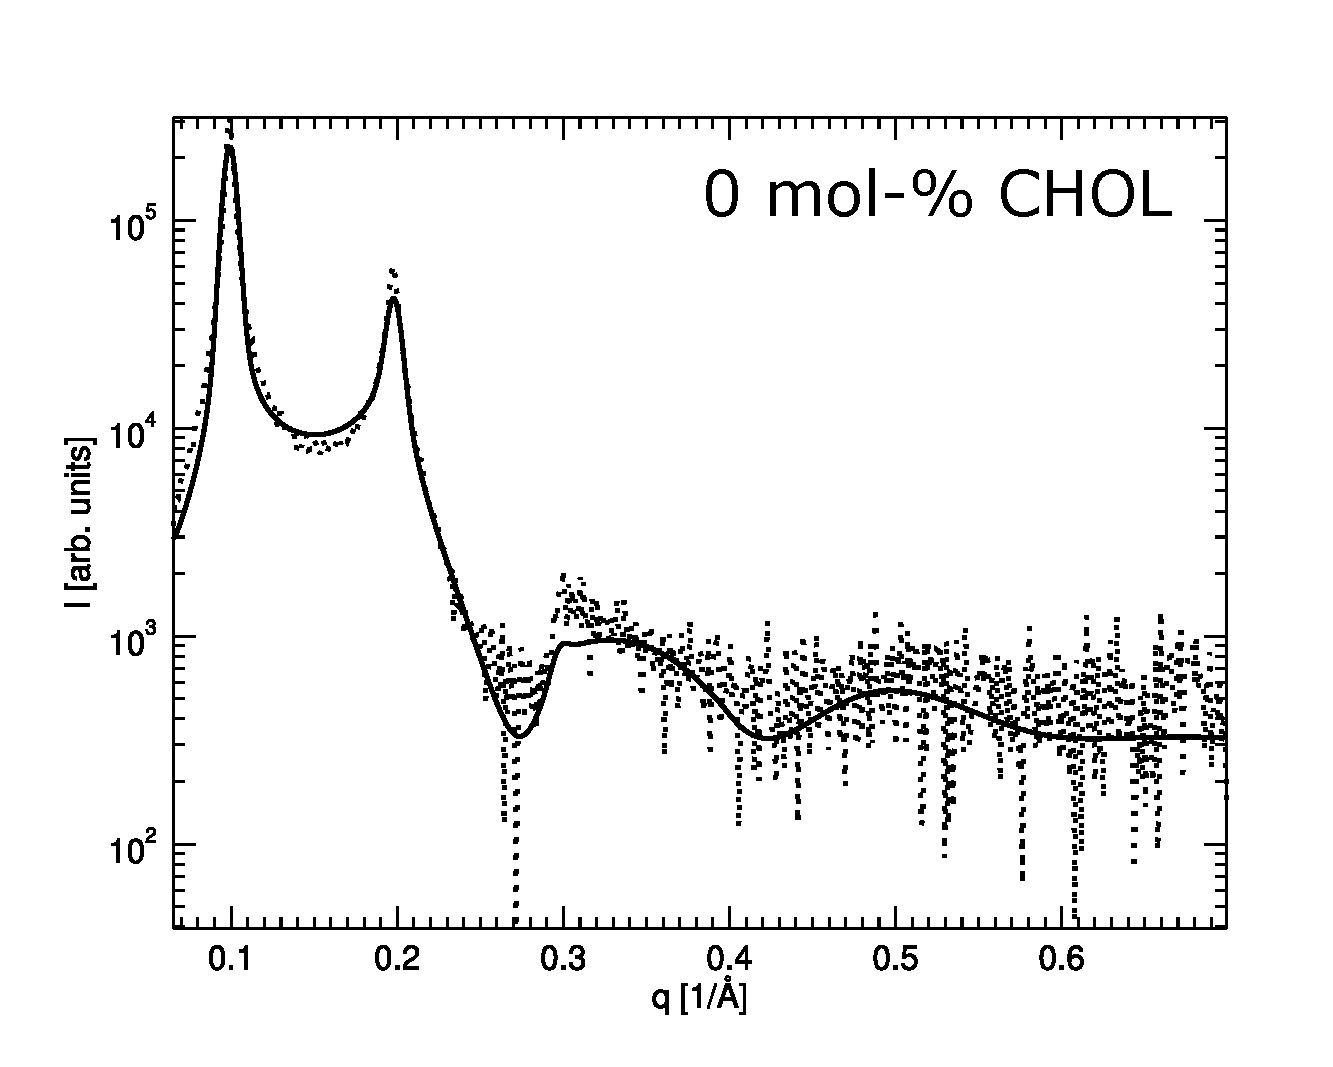
\includegraphics[width=0.45\linewidth]{../FIGS/scatt0.pdf}
    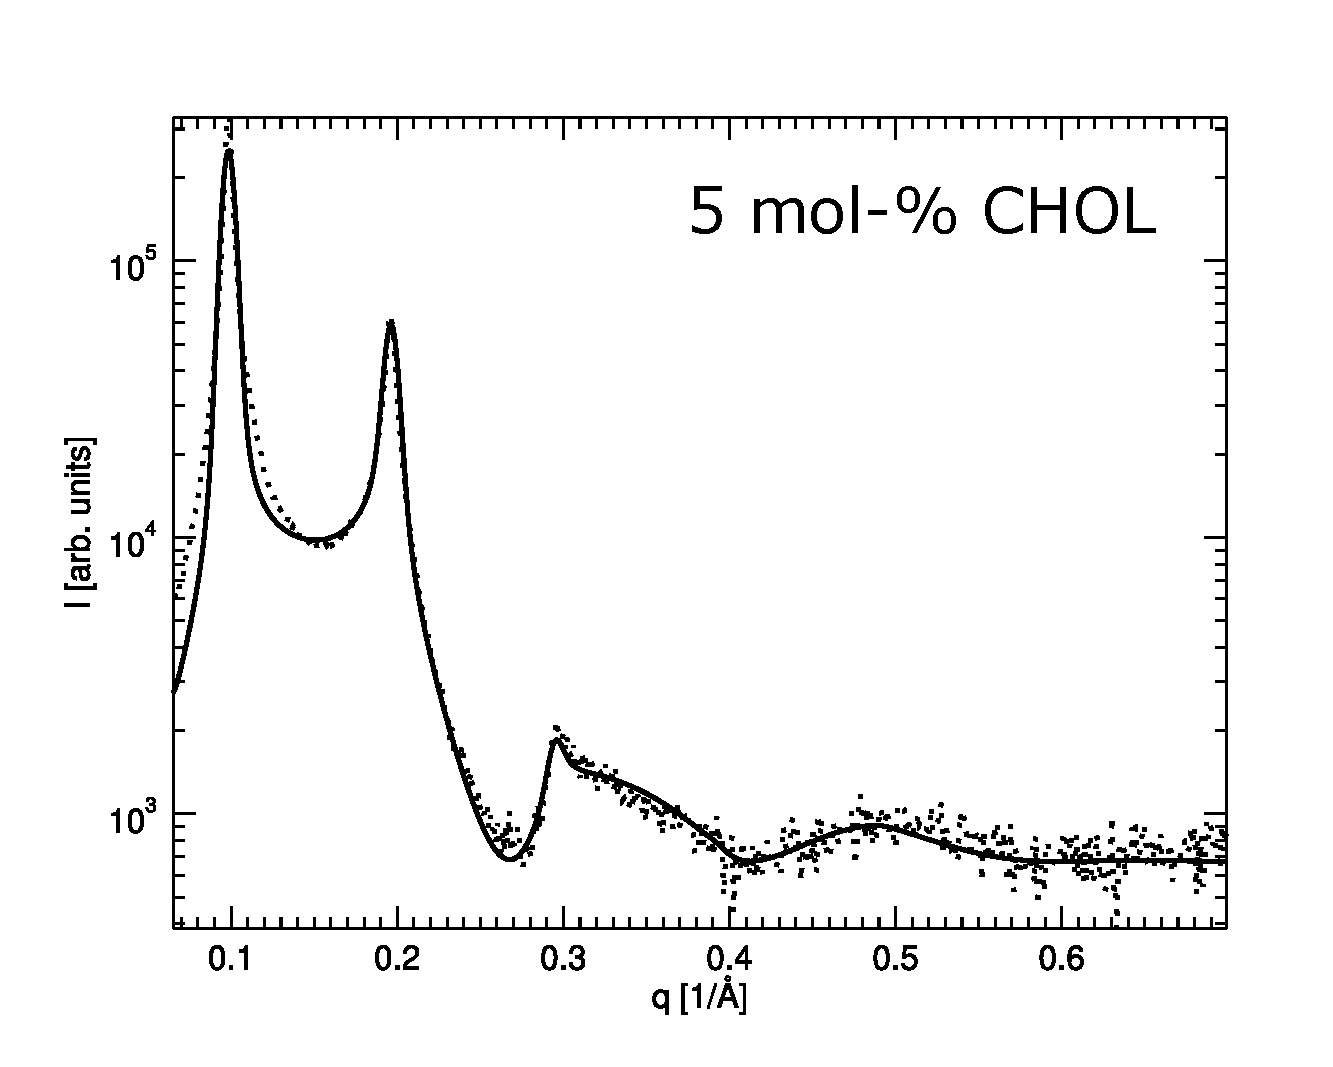
\includegraphics[width=0.45\linewidth]{../FIGS/scatt5.pdf}\\
    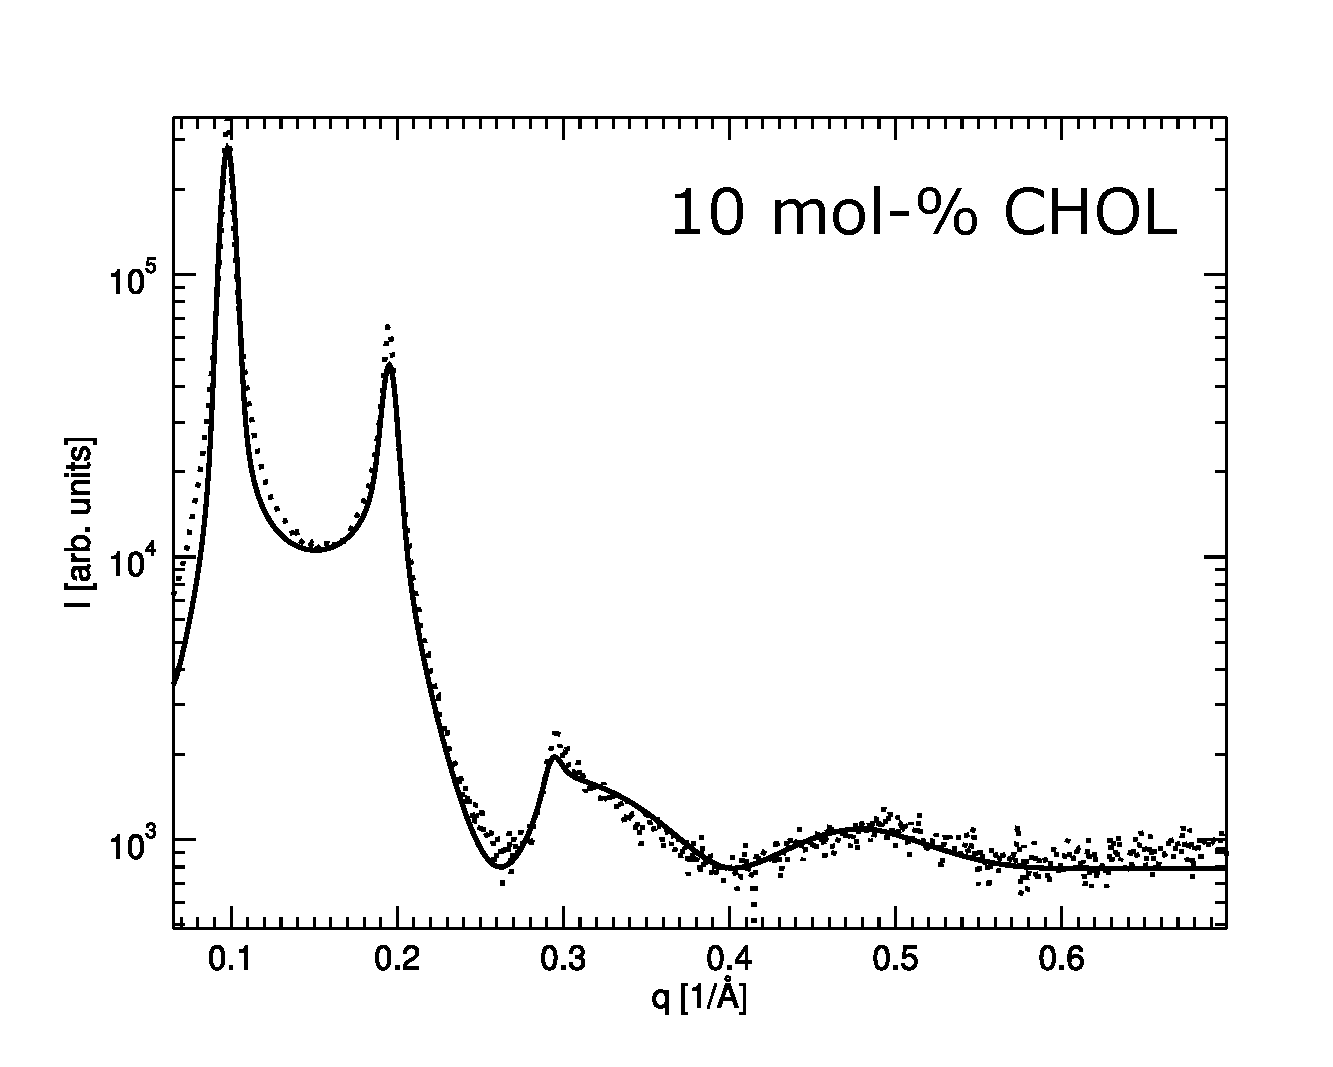
\includegraphics[width=0.45\linewidth]{../FIGS/scatt10.pdf}
    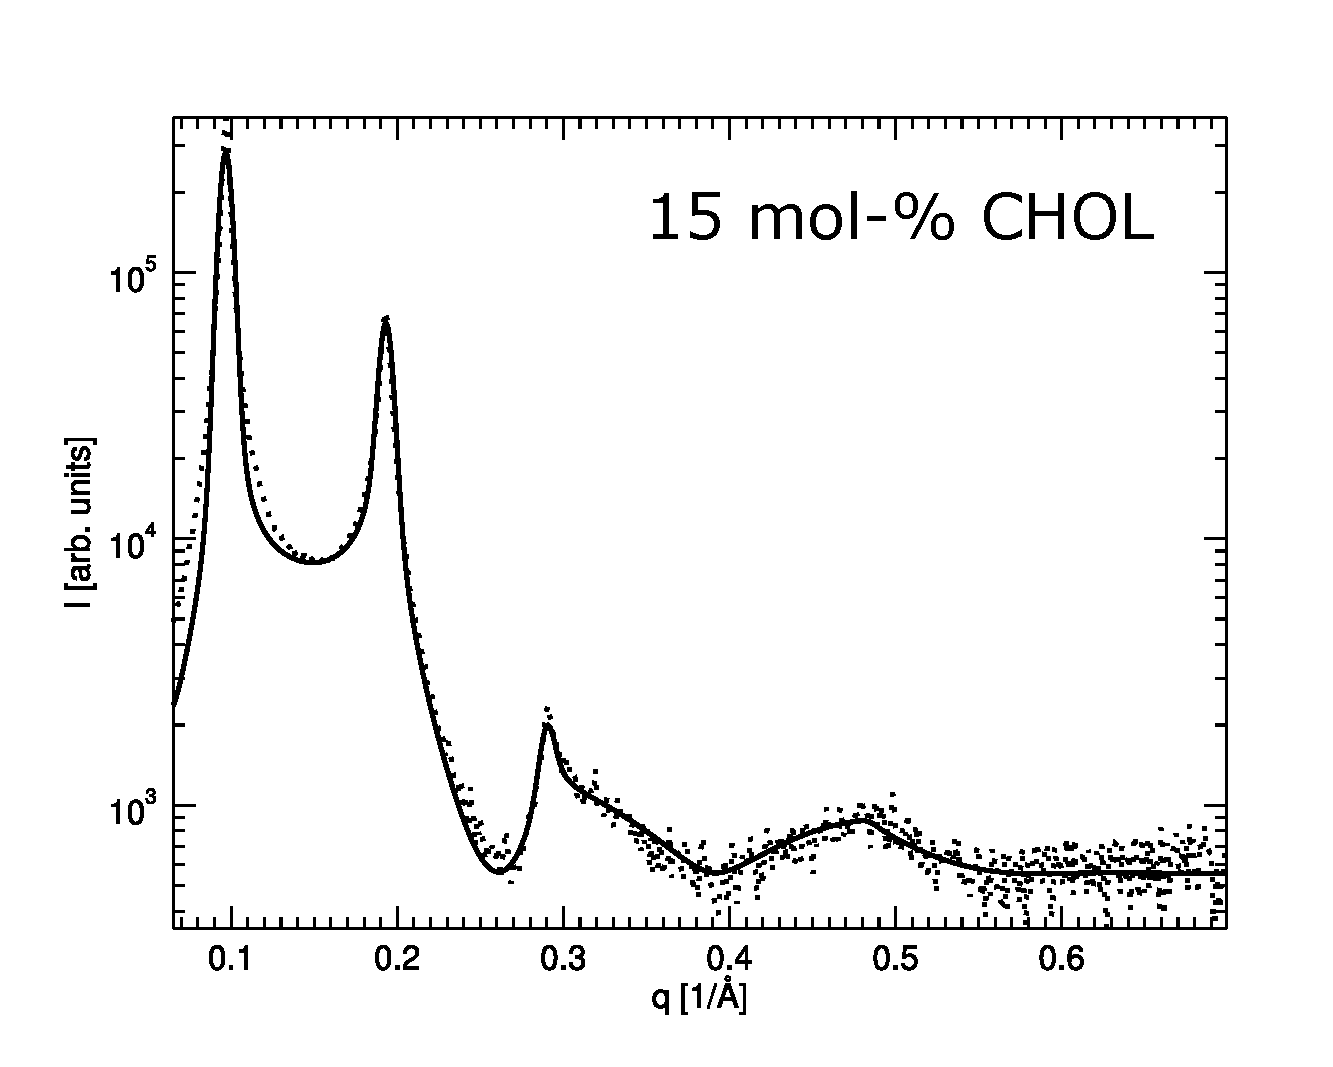
\includegraphics[width=0.45\linewidth]{../FIGS/scatt15.pdf}\\
    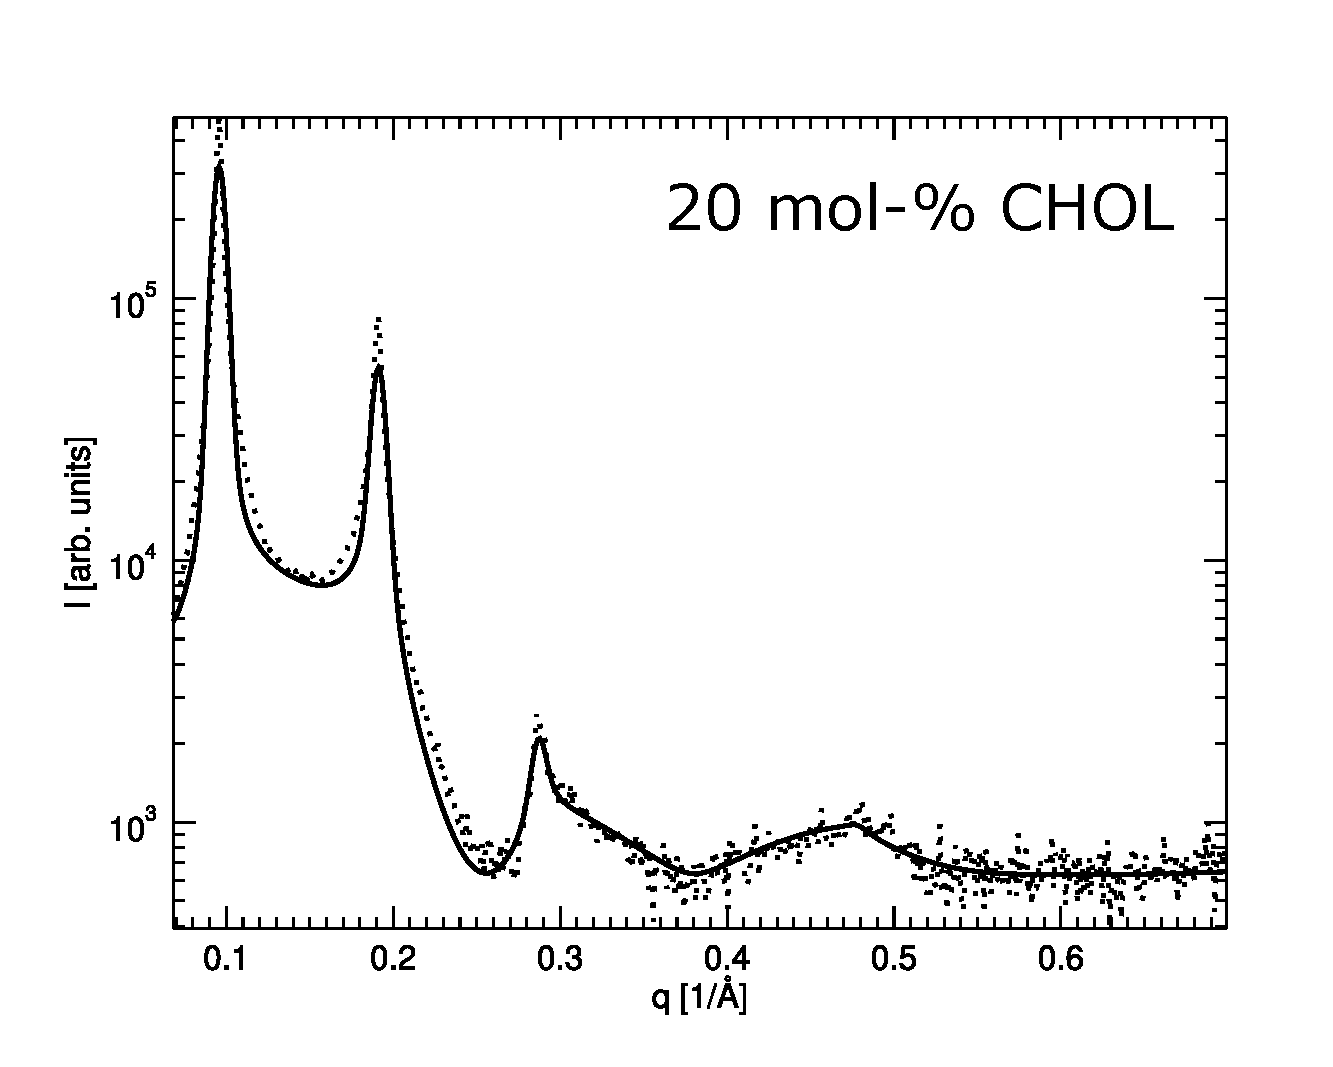
\includegraphics[width=0.45\linewidth]{../FIGS/scatt20.pdf}
    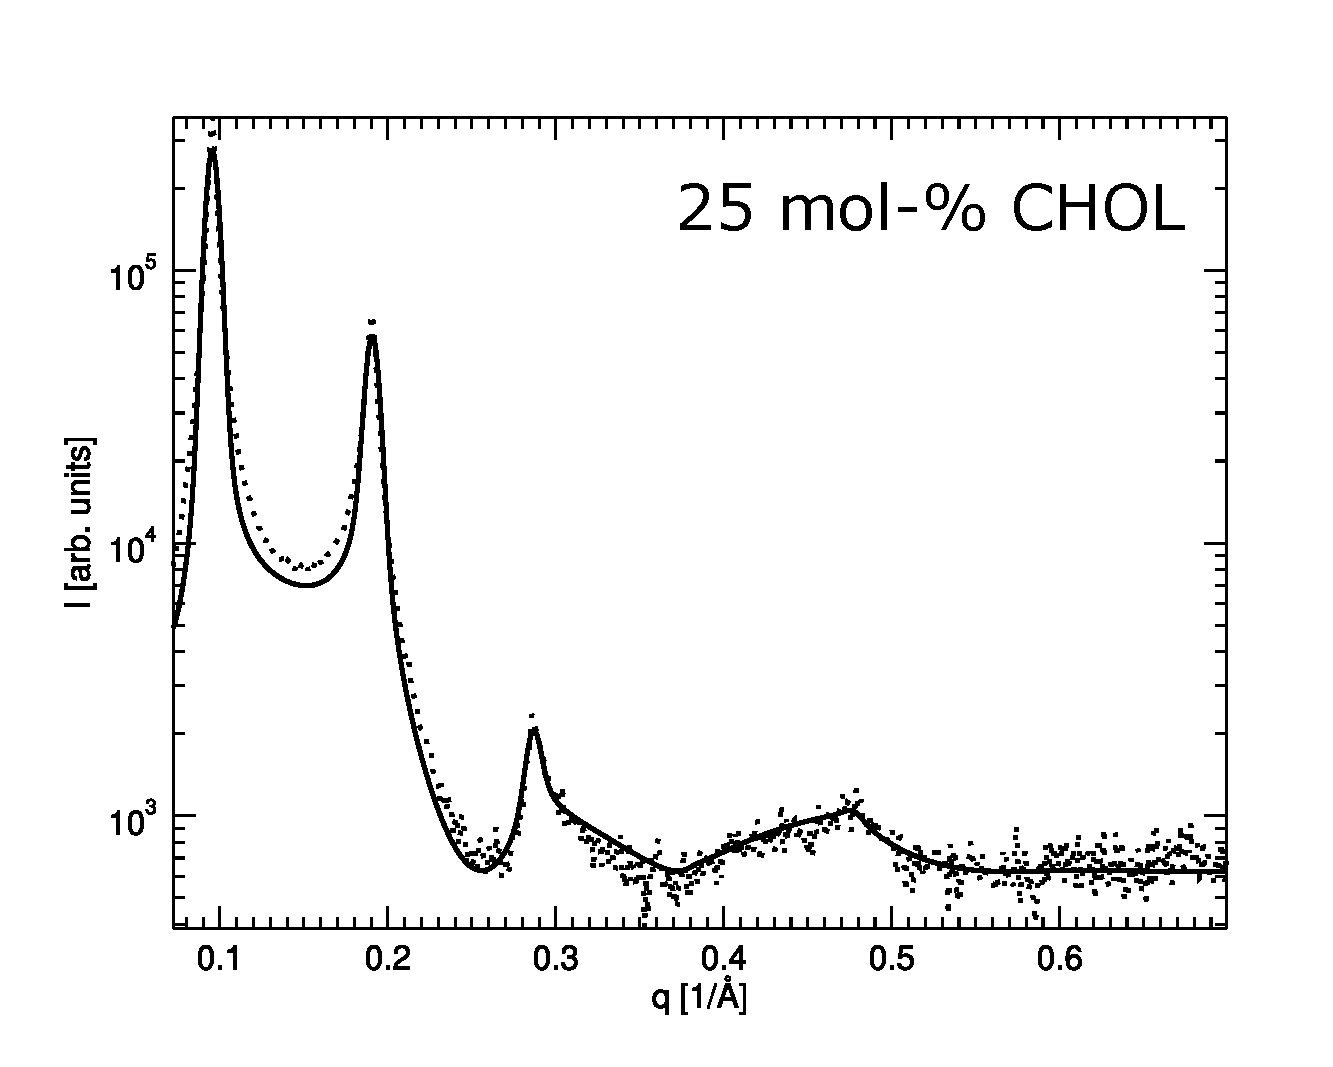
\includegraphics[width=0.45\linewidth]{../FIGS/scatt25.pdf}
    \caption{Scattering intensities from X-ray scattering experiments with various concentrations of cholesterol. More data are shown in the next figure.}
    \label{SIfig:scattering1}
\end{figure}

\clearpage

\begin{figure}[htb!]
    \centering
    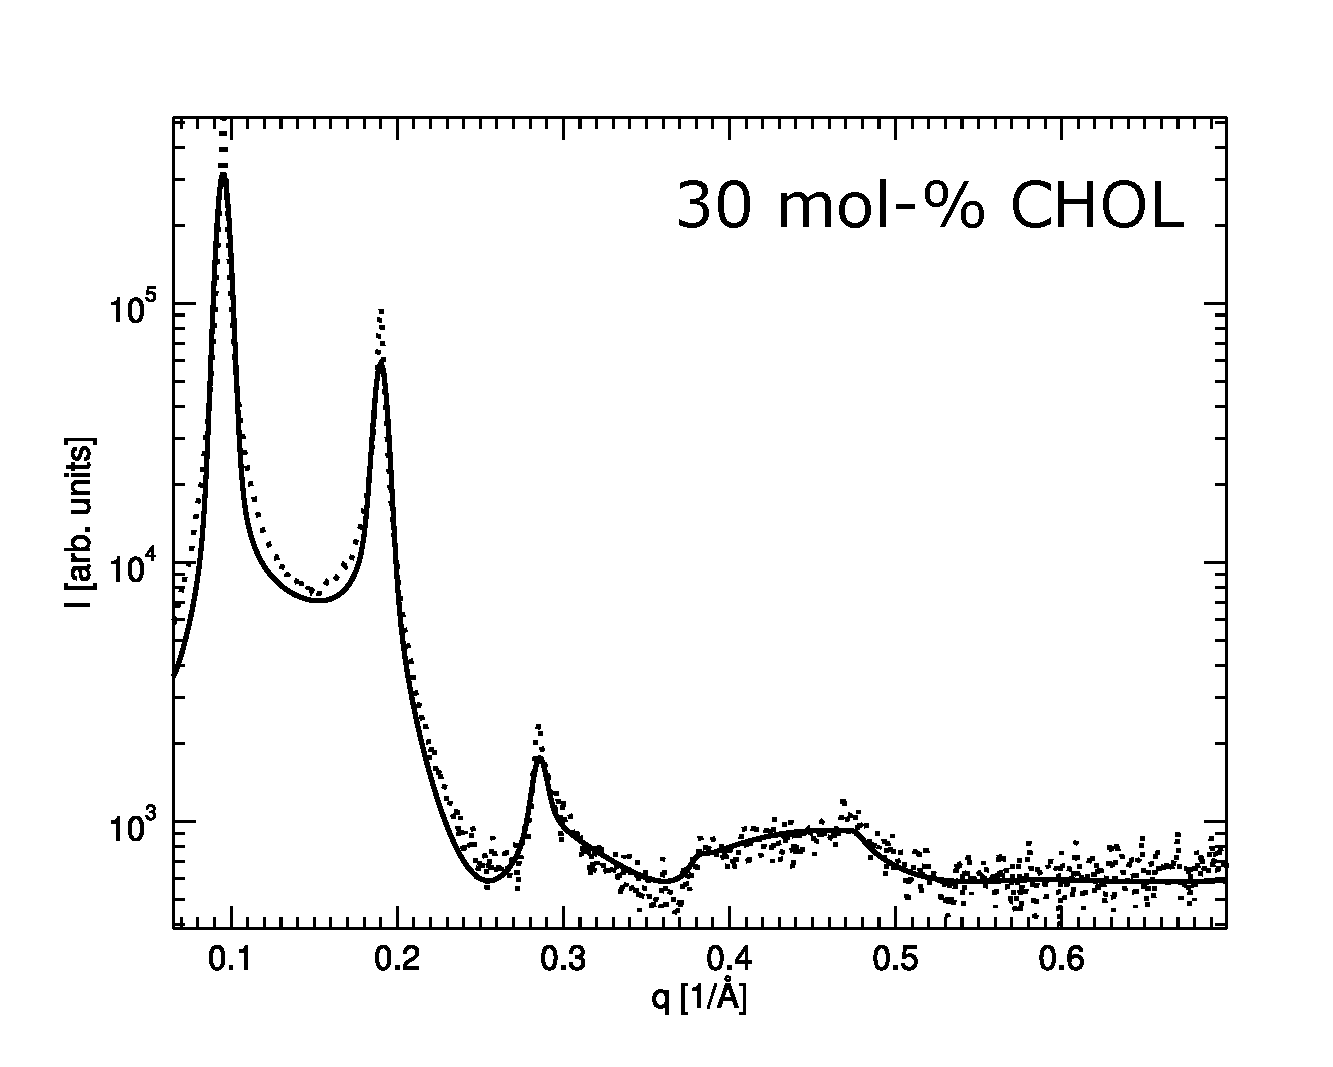
\includegraphics[width=0.45\linewidth]{../FIGS/scatt30.pdf}
    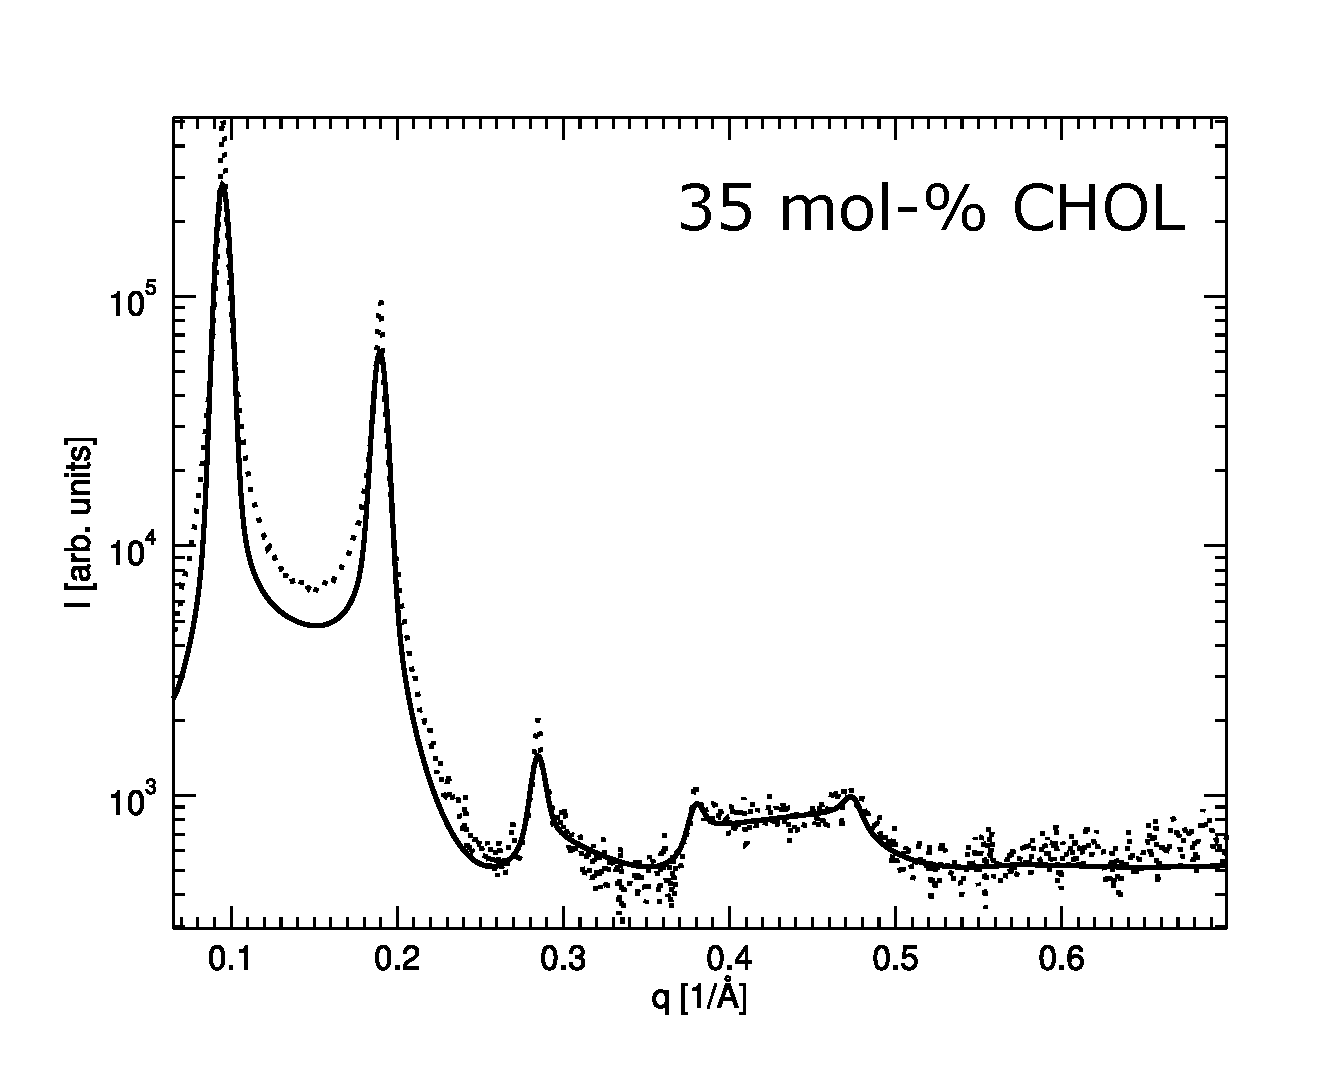
\includegraphics[width=0.45\linewidth]{../FIGS/scatt35.pdf}\\
    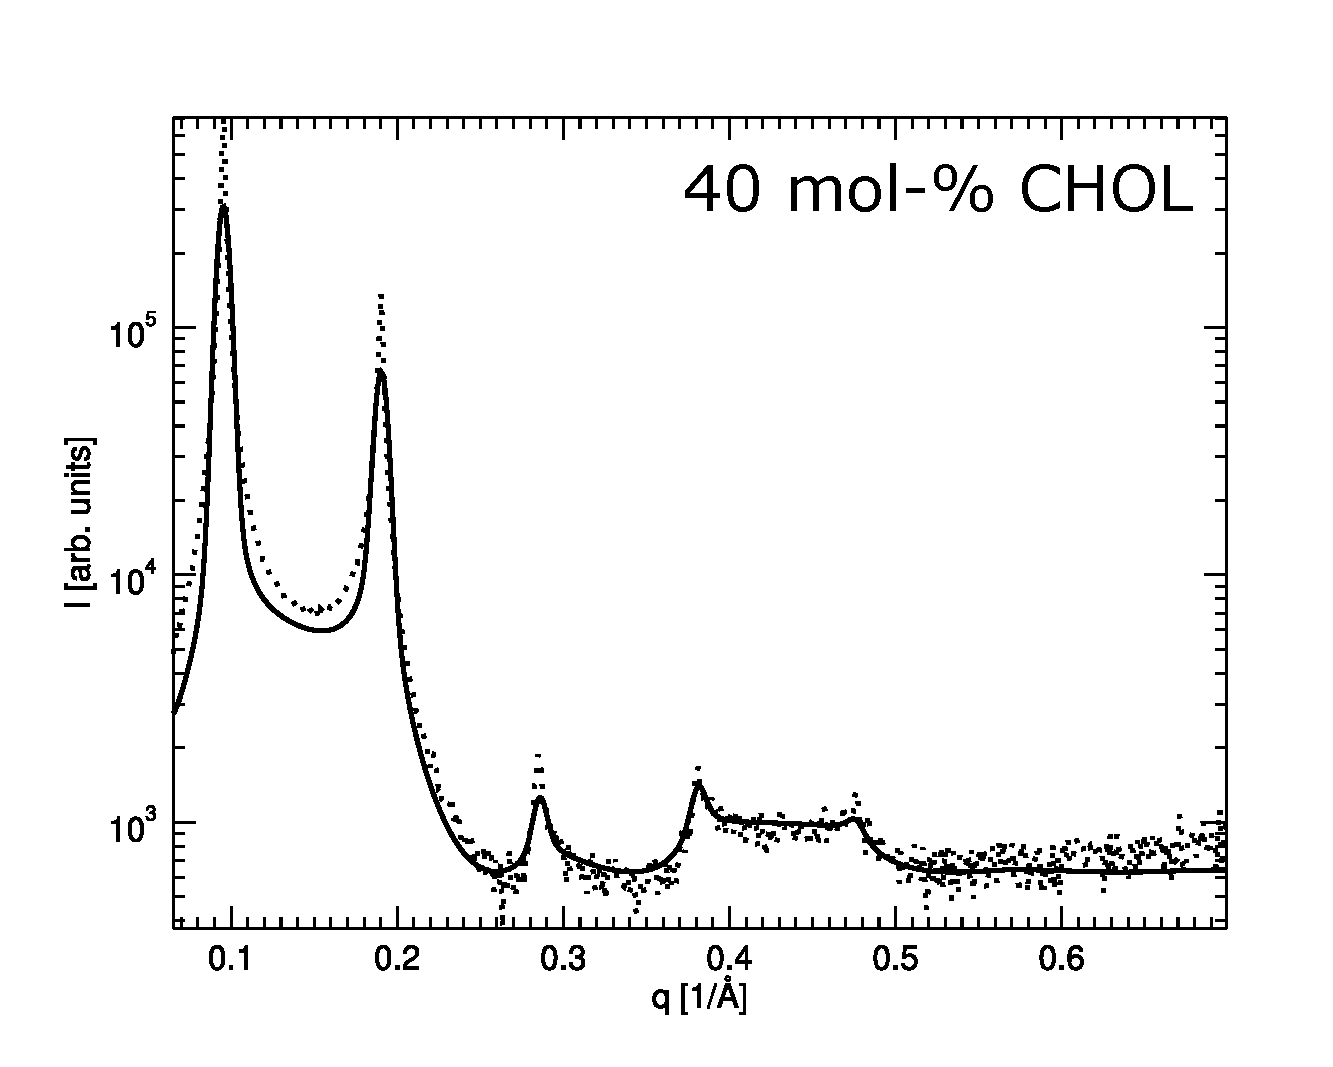
\includegraphics[width=0.45\linewidth]{../FIGS/scatt40.pdf}
    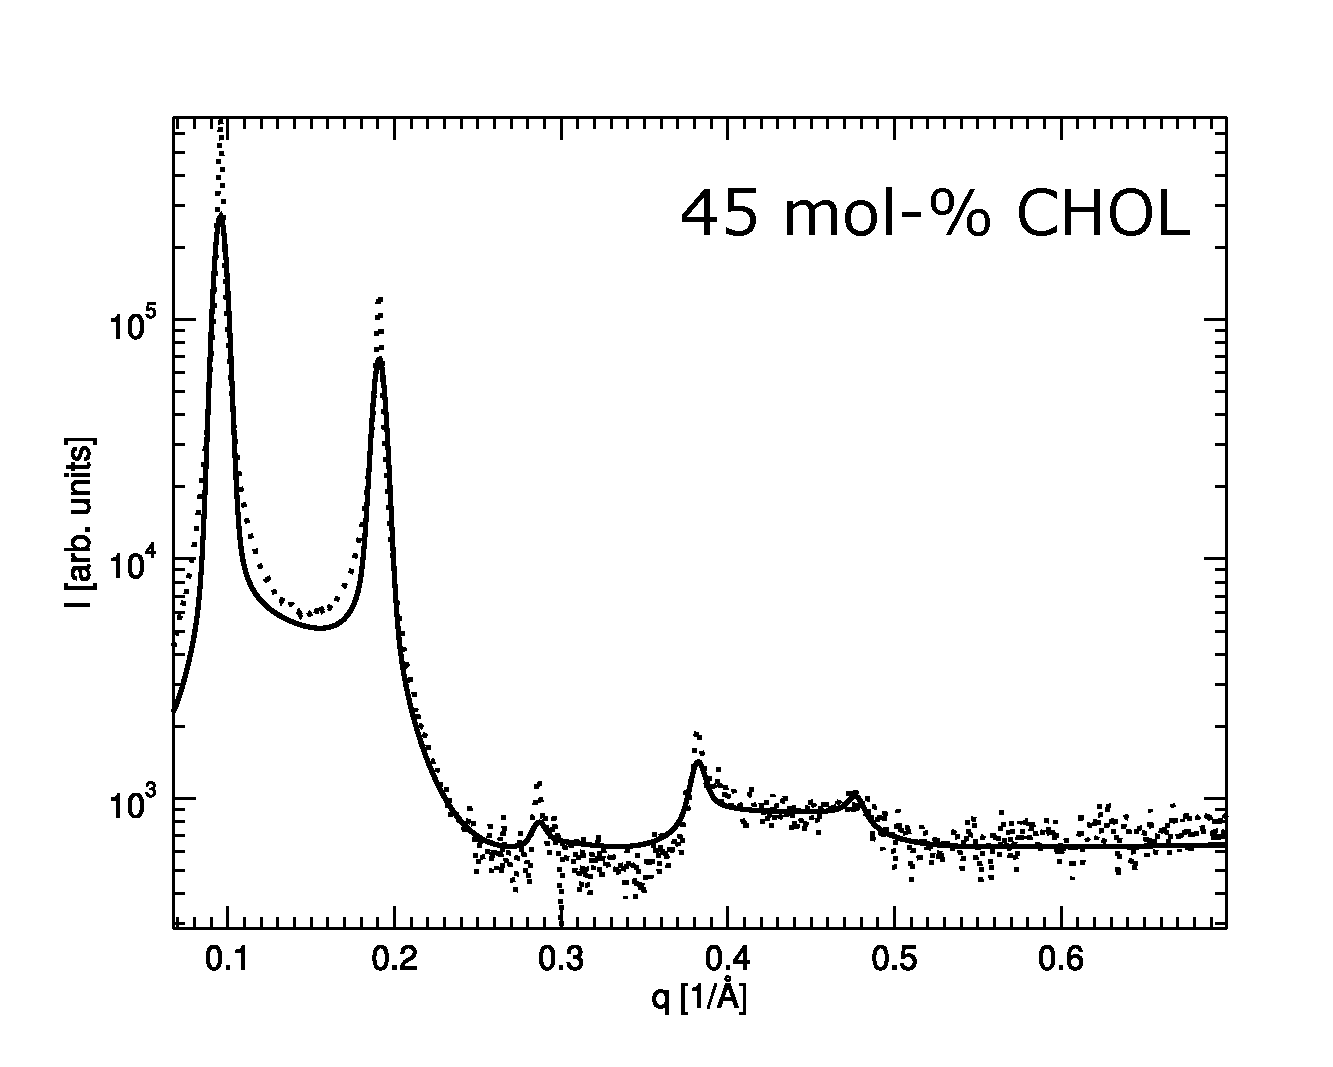
\includegraphics[width=0.45\linewidth]{../FIGS/scatt45.pdf}\\
    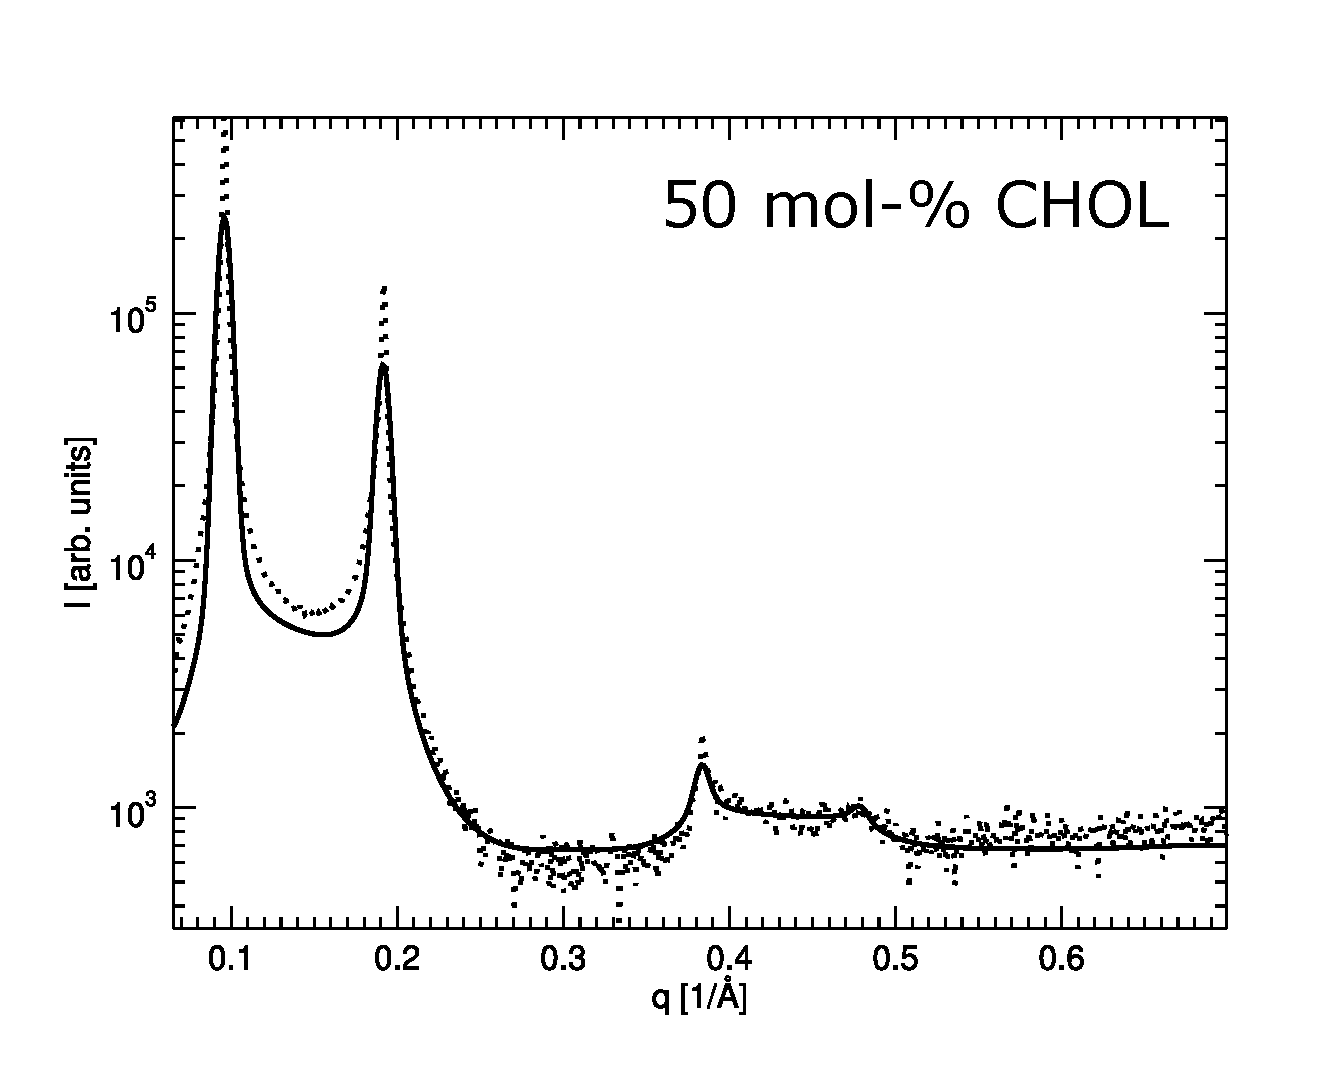
\includegraphics[width=0.45\linewidth]{../FIGS/scatt50.pdf}
    \caption{Scattering intensities from X-ray scattering experiments with various concentrations of cholesterol. More data are shown in the previous figure.}
    \label{SIfig:scattering2}
\end{figure}

\clearpage

\subsection{Form Factors \& Electron Density Profiles}

\begin{figure}[htb!]
    \centering
    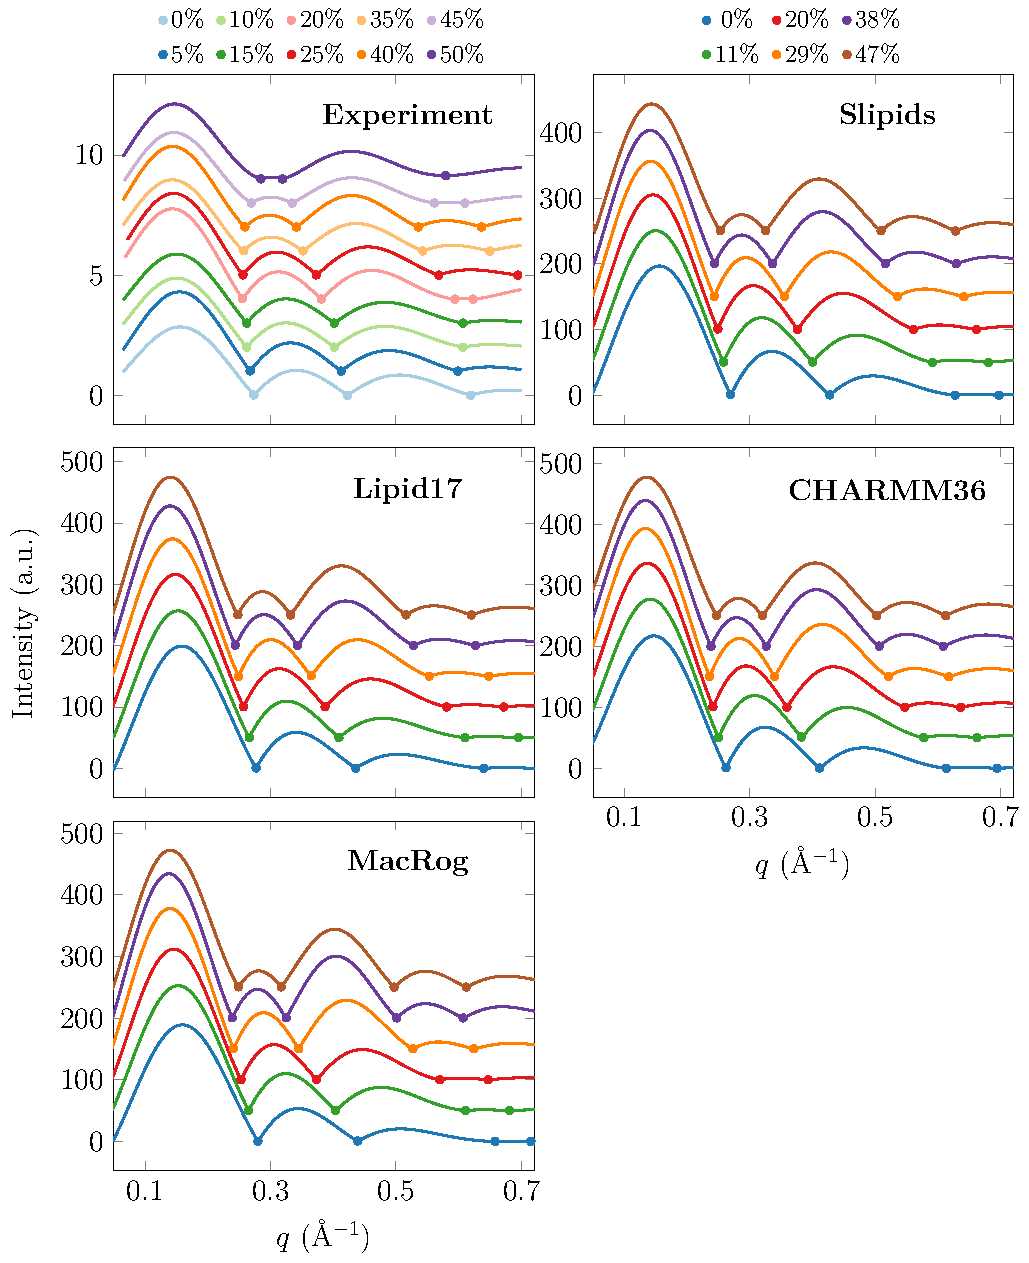
\includegraphics[width=0.86\linewidth]{../FIGS/scattering.pdf}
    \caption{\label{SIfig:scattering}%
     \textbf{Scattering intensities as a function of scattering vector from experiments and simulations.} Each of the profiles is shifted vertically with respect to the previous one, by 1 for the experimental profiles and by 50 for the computational ones. The minima are marked by filled circles to guide the eye.
    }
\end{figure}

\begin{figure}[htb!]
    \centering
    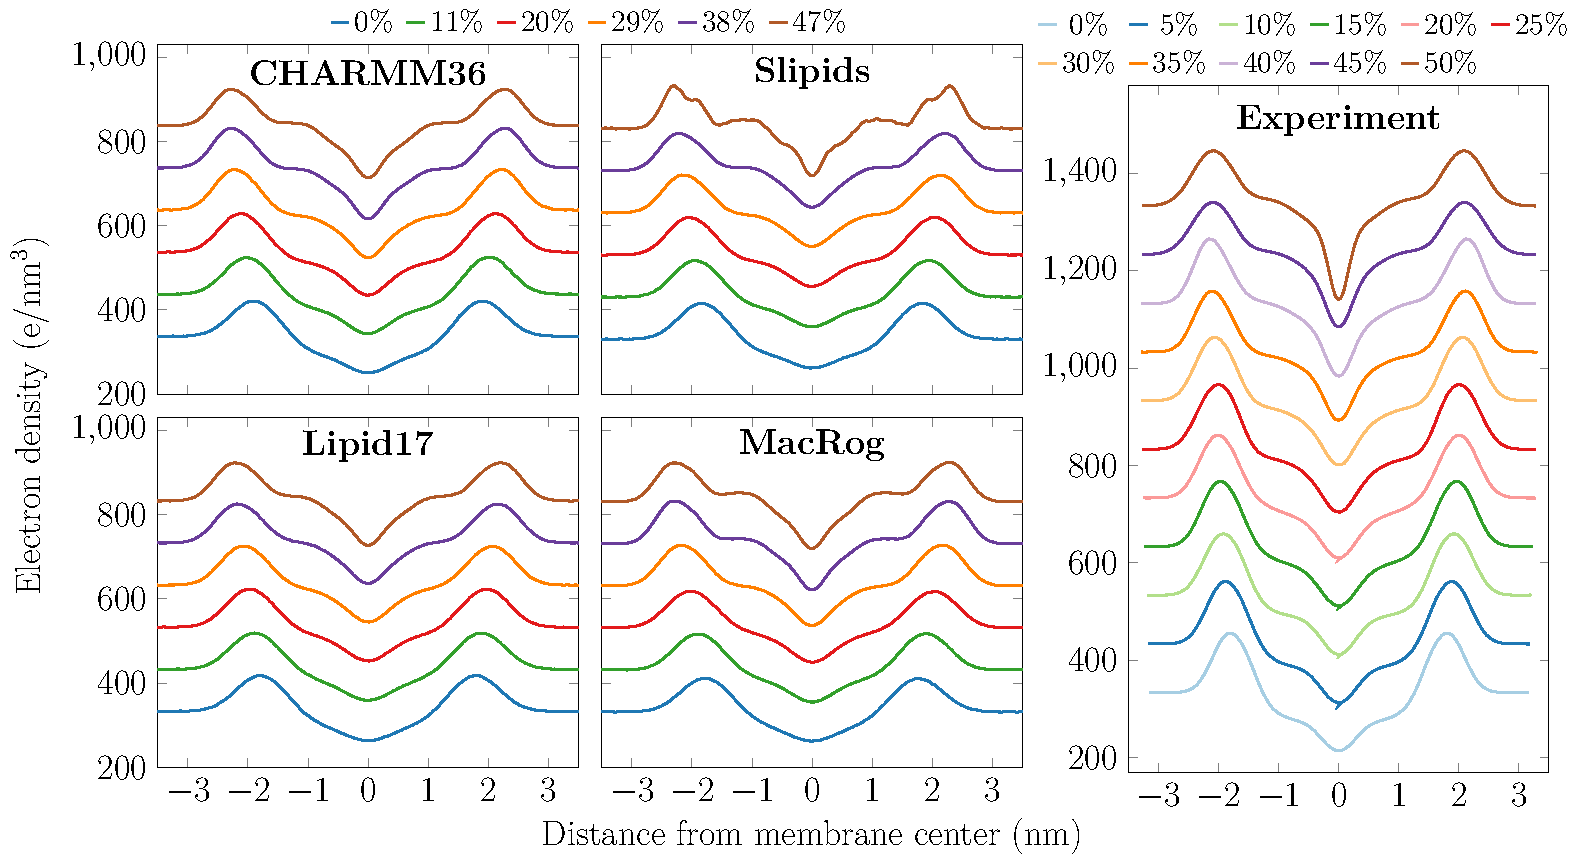
\includegraphics[width=\linewidth]{../FIGS/densityprofiles.pdf}
    \caption{\label{SIfig:densprofs}%
    \textbf{Electron density profiles.}
    Each of the profiles is shifted vertically with respect to the previous one by 100 units.
    }
\end{figure}

\clearpage
\subsection{Order Parameters}

\begin{figure}[htb!]
    \centering
    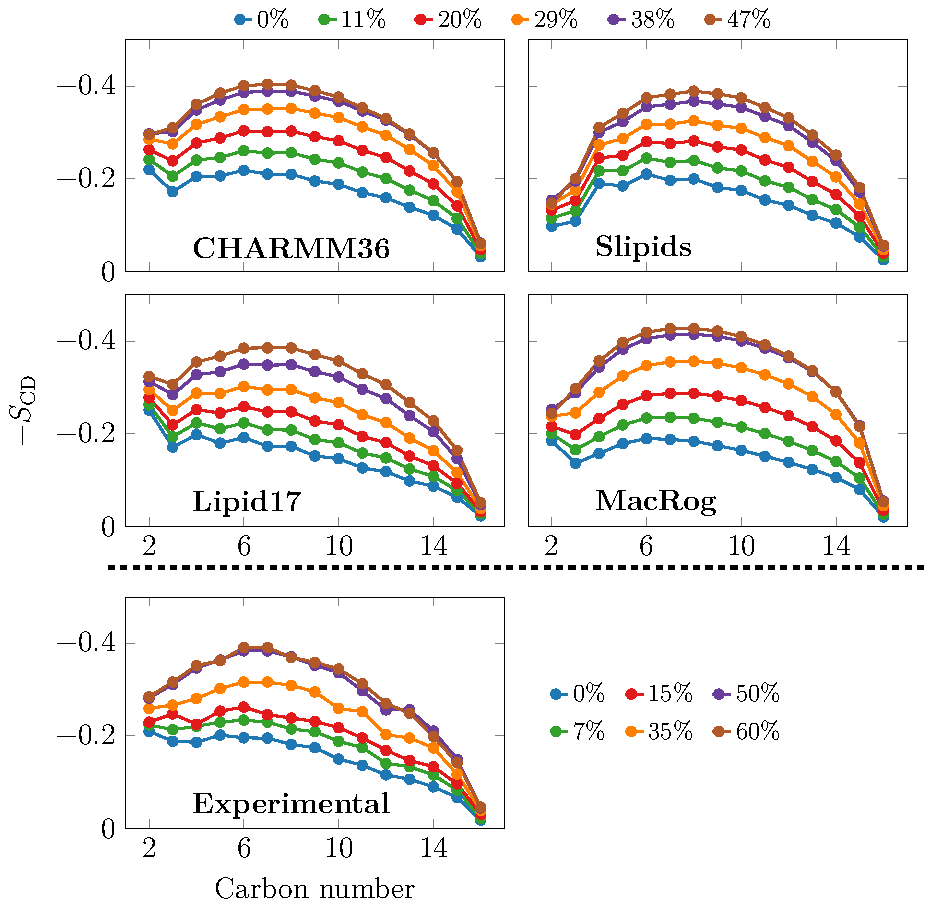
\includegraphics[width=0.9\linewidth]{../FIGS/palmitate.pdf}
    \caption{\label{SIfig:palmitate}%
     \textbf{Effect of cholesterol on the acyl chain order parameters of the POPC $sn$-1 (palmitate) chain.}
     The legend at the top corresponds to all simulations, and the one at the bottom to the experiments.
    }
\end{figure}

\begin{figure}[htb!]
    \centering
    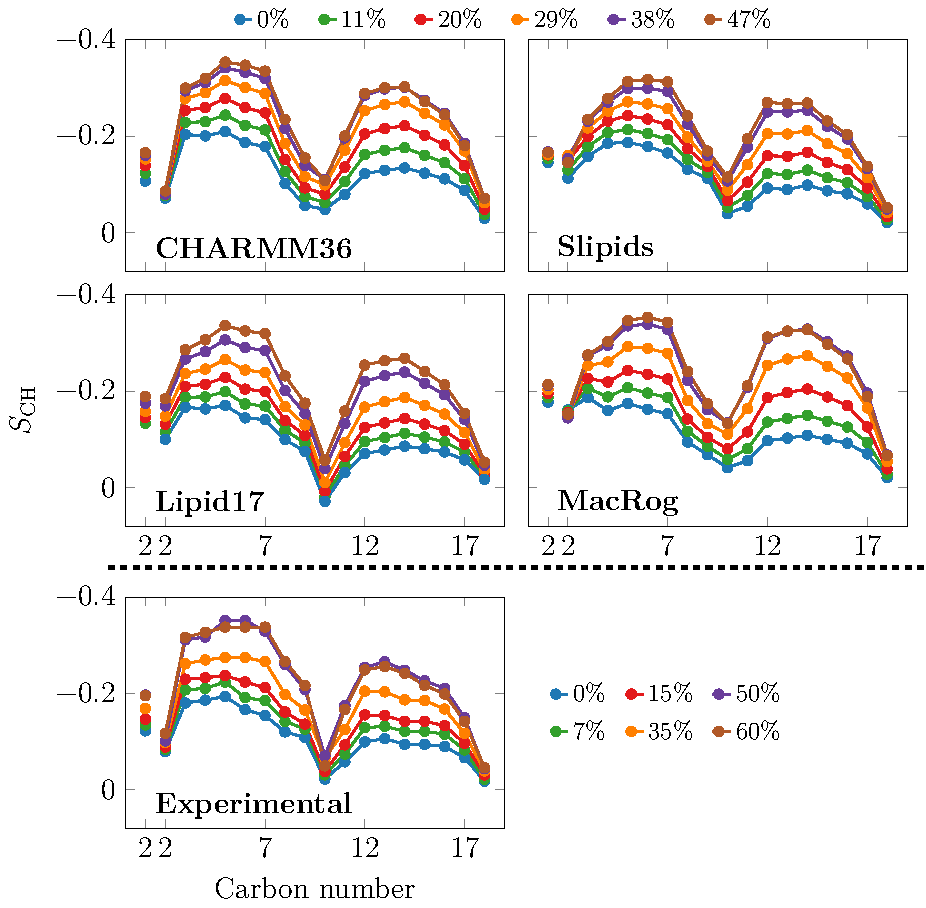
\includegraphics[width=0.9\linewidth]{../FIGS/oleate.pdf}
    \caption{\label{SIfig:oleate}%
     \textbf{Effect of cholesterol on the acyl chain order parameters of the POPC $sn$-2 (oleate) chain.}
     The legend at the top corresponds to all simulations, and the one at the bottom to the experiments. Since the order parameters measured for the two hydrogens bound to the C2 carbon differ, they are both shown in the plots.
    }
\end{figure}

\begin{figure}[htb!]
    \centering
    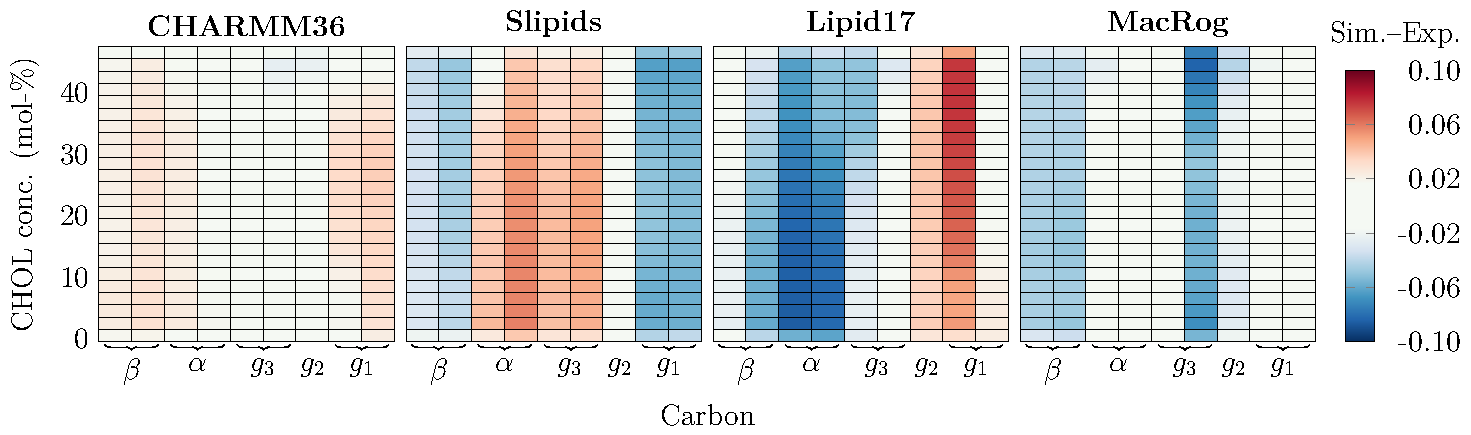
\includegraphics[width=\linewidth]{../FIGS/OP_headgroup.pdf}
    \caption{\label{SIfig:headgroups}%
     \textbf{The deviation of POPC head group parameters from experimental values as a function of CHOL concentration.}
    }
\end{figure}

\clearpage
\subsection{Dynamic Properties}

\begin{figure}[htb!]
    \centering
    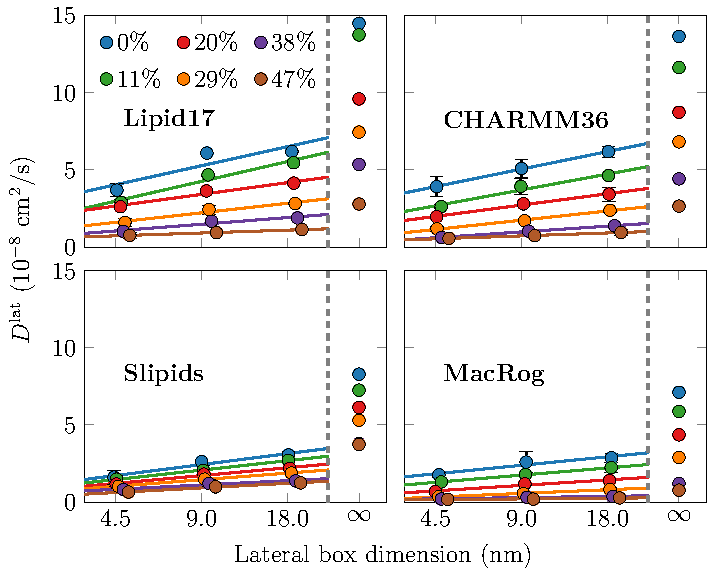
\includegraphics[width=0.9\linewidth]{../FIGS/d_vs_size.pdf}
    \caption{\label{SIfig:dvssize}%
    \textbf{Dependence of lateral diffusion coefficients on simulation box size.} The values calculated for the lipid centres of mass with \texttt{gmx msd} after eliminating leaflet drift. The values for the three system sizes are shown as markers together with fits of Eq.~\eqref{eq:sdlatpbc}. The values extrapolated to infinite system sizes are also shown in the separate column. 
    }
\end{figure}

\begin{figure}[htb!]
    \centering
    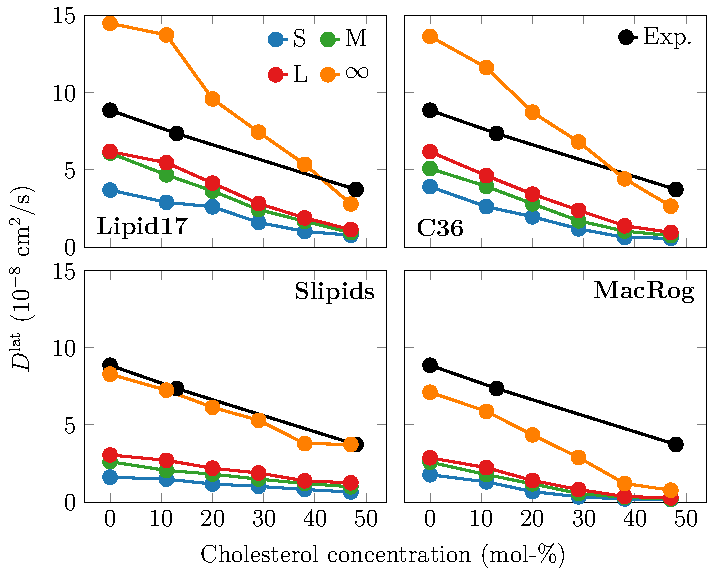
\includegraphics[width=0.9\linewidth]{../FIGS/d_vs_chol.pdf}
    \caption{\label{SIfig:dvschol}%
     \textbf{Dependence of lateral diffusion coefficients on cholesterol concentration.} Data are shown for all system sizes; small (S), medium (M), and large (L). The values extrapolated to infinity are shown as well ($\infty$). Experimental measured at two hydration levels, 30 m-\% and 55-\% of water \cite{filippov2003effect,filippov2003influence}.
    }
\end{figure}

\clearpage
\subsection{Finite-Size Effects}

\begin{figure}[htb!]
    \centering
    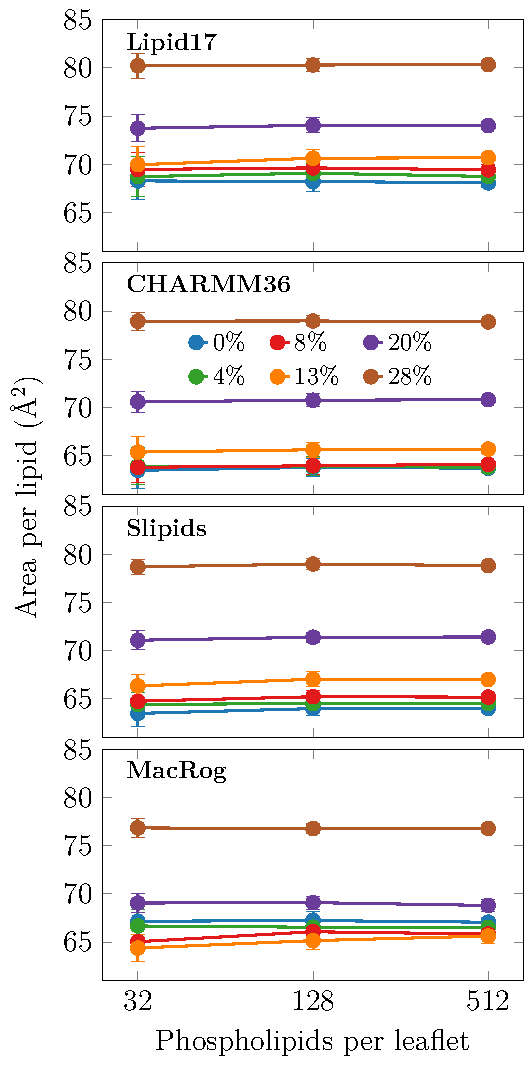
\includegraphics[width=8.7cm]{../FIGS/apl_vs_size.pdf}
    \caption{\label{SIfig:aplvssize}%
     \textbf{Dependence of area per lipid on simulation box size.} Area per lipid is calculated by dividing the membrane area by the number of lipids in one leaflet. Error bars show standard error extracted using block averaging in \texttt{gmx analyze}.
    }
\end{figure}

\begin{figure}[htb!]
    \centering
    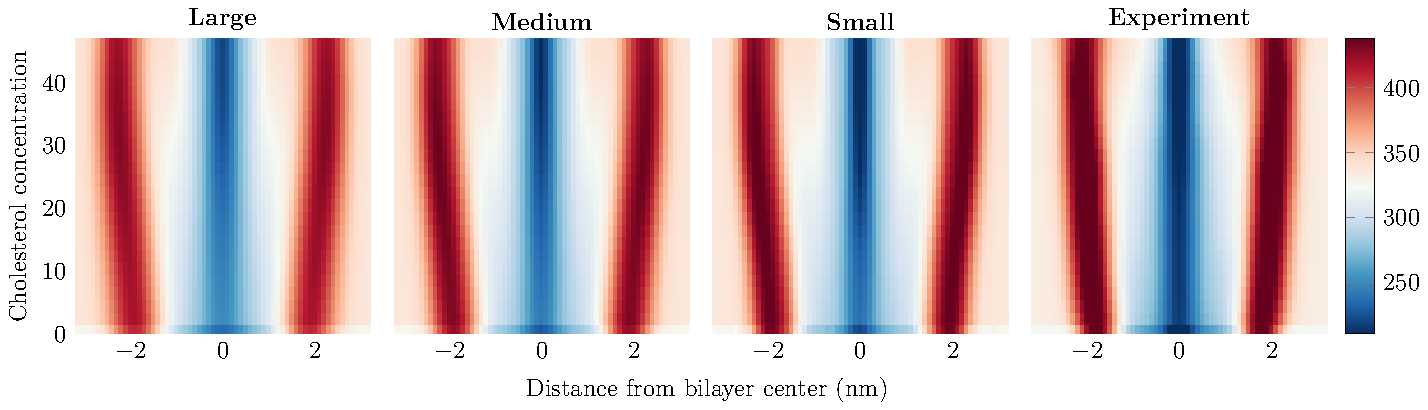
\includegraphics[width=\linewidth]{../FIGS/densityprofiles_size.pdf}
    \caption{\label{SIfig:densprofssize}%
    \textbf{Effect of system size on the density profiles.}
    Membrane undulations are larger in the larger systems, which leads to the smearing of the electron density profiles. Here, data are shown for CHARMM36 in the large (1024 POPC in total), medium (256 POPC in total), or small (64 POPC in total) systems. The experimental electron density profile is shown for comparison.
    }
\end{figure}

\clearpage


\bibliography{refs.bib}

\end{document}